\label{sec:methods}
\section{Methods and Materials}

The design and the implementation of the nuclear reactor were carried out using MCNP5.1 run both locally, as well as remotely on servers to verify results.  The design was approached in a "bottom-up" faction. This meant that the reactor's core was designed and tested first. After this, the surrounding material, as well as its geometry, were designed and tested for optimal neutron reflectivity. Finally, the output chamber was added with an FMESH tally running the neutron counts. This approach allowed us to incrementally structure the reactor and catch any errors in their early stages.\\

\subsection{Core}

After considering several variations of breeder reactors, all of which were Thorium based, the element of choice for the core was Uranium-235. Due to safety concerns for real-life implementation, its purity could not be 100\%, however reactivity calculations were carried out to understand initial core sizes at this percentage. Uranium-235's value in core composition was decreased to 19\% after initial tests. Again, this was done to address safety concerns while operating the reactor. The rest of the core, mainly 81\%, was made up of Graphite for neutron moderation.\\

The core was designed in the following way. Two layers of Uranium-235 blocks are arranged in a 2 by 4 grid. In between each block and both layers, the Graphite acts as the neutron moderator. The structure can be seen in figure \ref{fig:core}.

\begin{figure}[!htbp]
\caption{Reactor core cross sections.}
\label{fig:core}
\centering
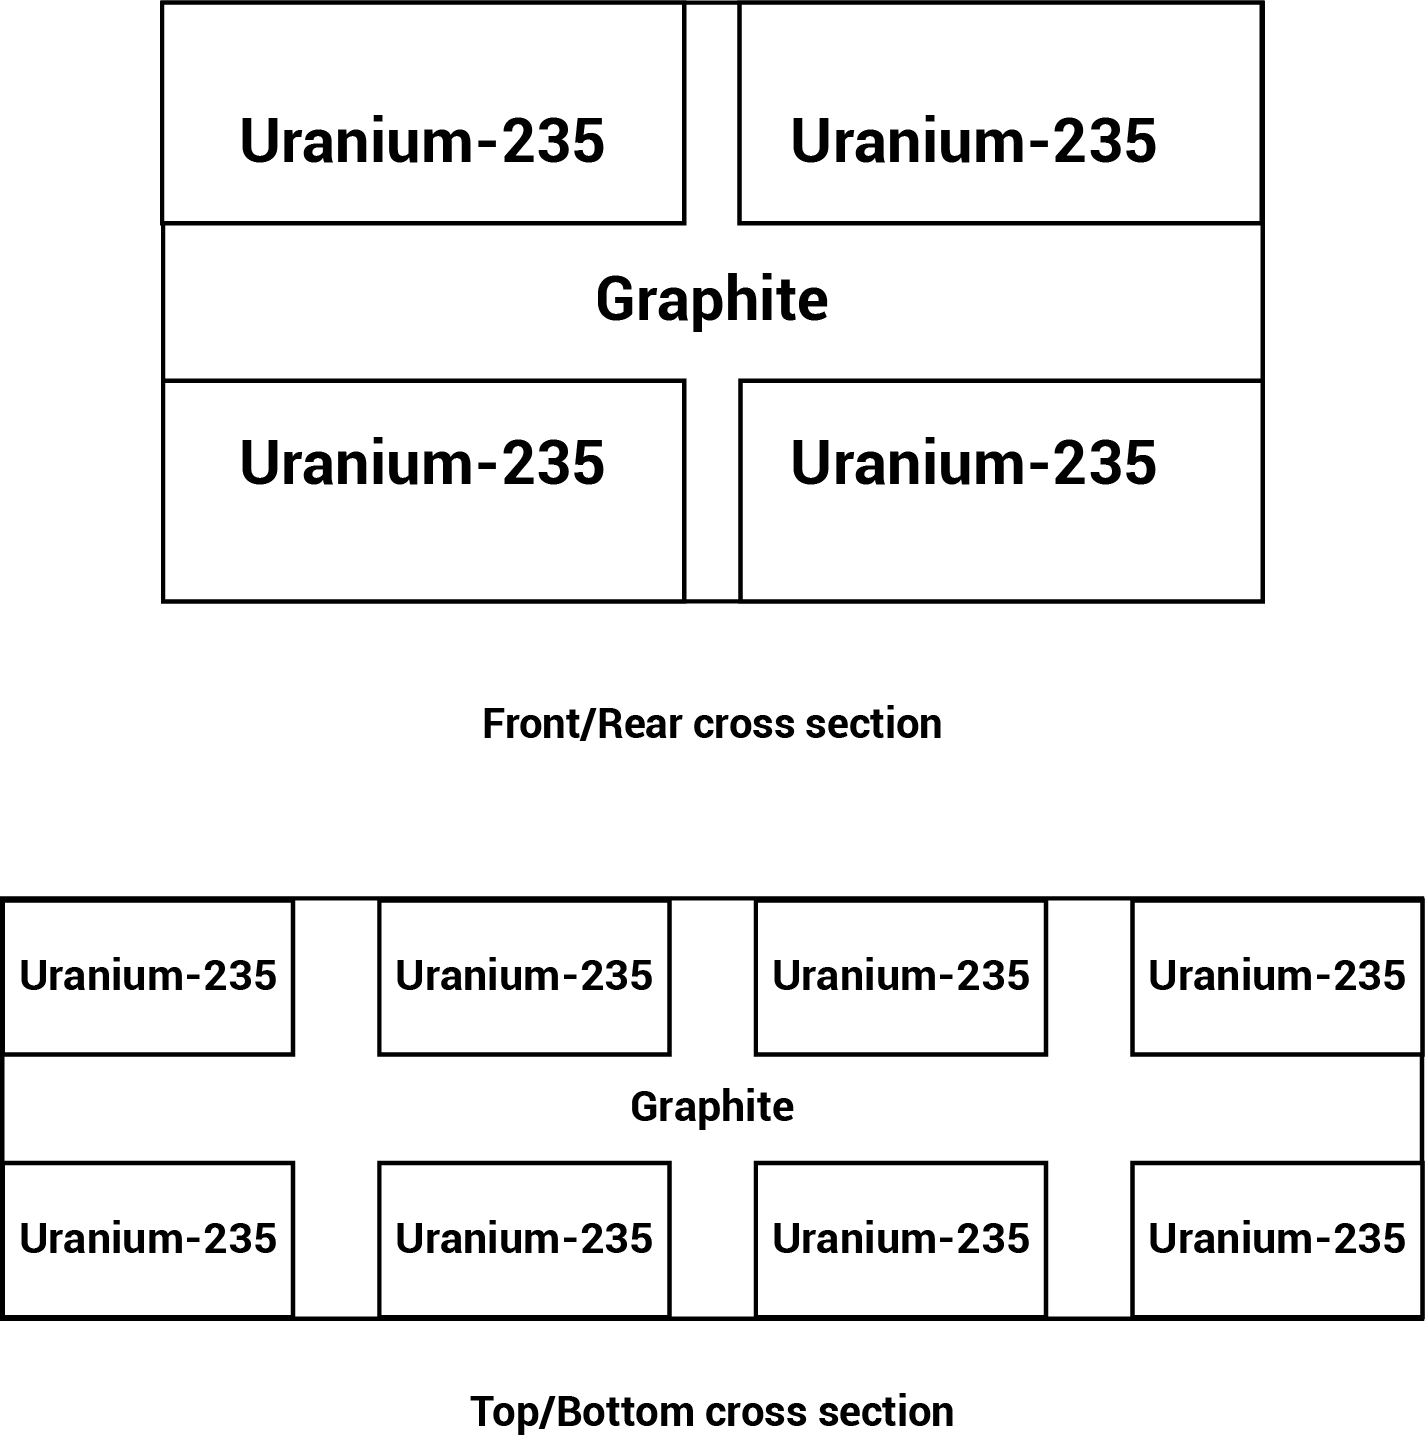
\includegraphics[width=0.5\textwidth]{core.png}
\end{figure}

With this structure, all of the emitted and absorbed neutrons will be regulated by the Graphite. The likelihood of a runaway reaction decreases due to the embedding of the Uranium blocks. For the reaction to be sustainable, the neutrons should be thermal, hence fast neutrons will not be captured and will not contribute to the fissions. Instead, they will be absorbed (along with excess particles) by the Graphite.\\

The structure of the core, however, can be simplified for the MCNP simulations and further power calculations. The complete block of Uranium and Graphite can be turned into one single block. As already stated, the composition of said block will be a 19\%-81\% split of Uranium-235 and Graphite. The dimensions and composition were chosen after running criticality simulations. More detailed information on the core's dimensions and criticalities can be found in section \ref{sec:results}.

\subsection{Shell}
\subsection{Chamber}
\subsection{Tally}